% \newpage
\section{Ablation Study}

%\subsection{Effect of Style Reward Learning (SRL). }




\begin{figure*}[!t]
    \centering
    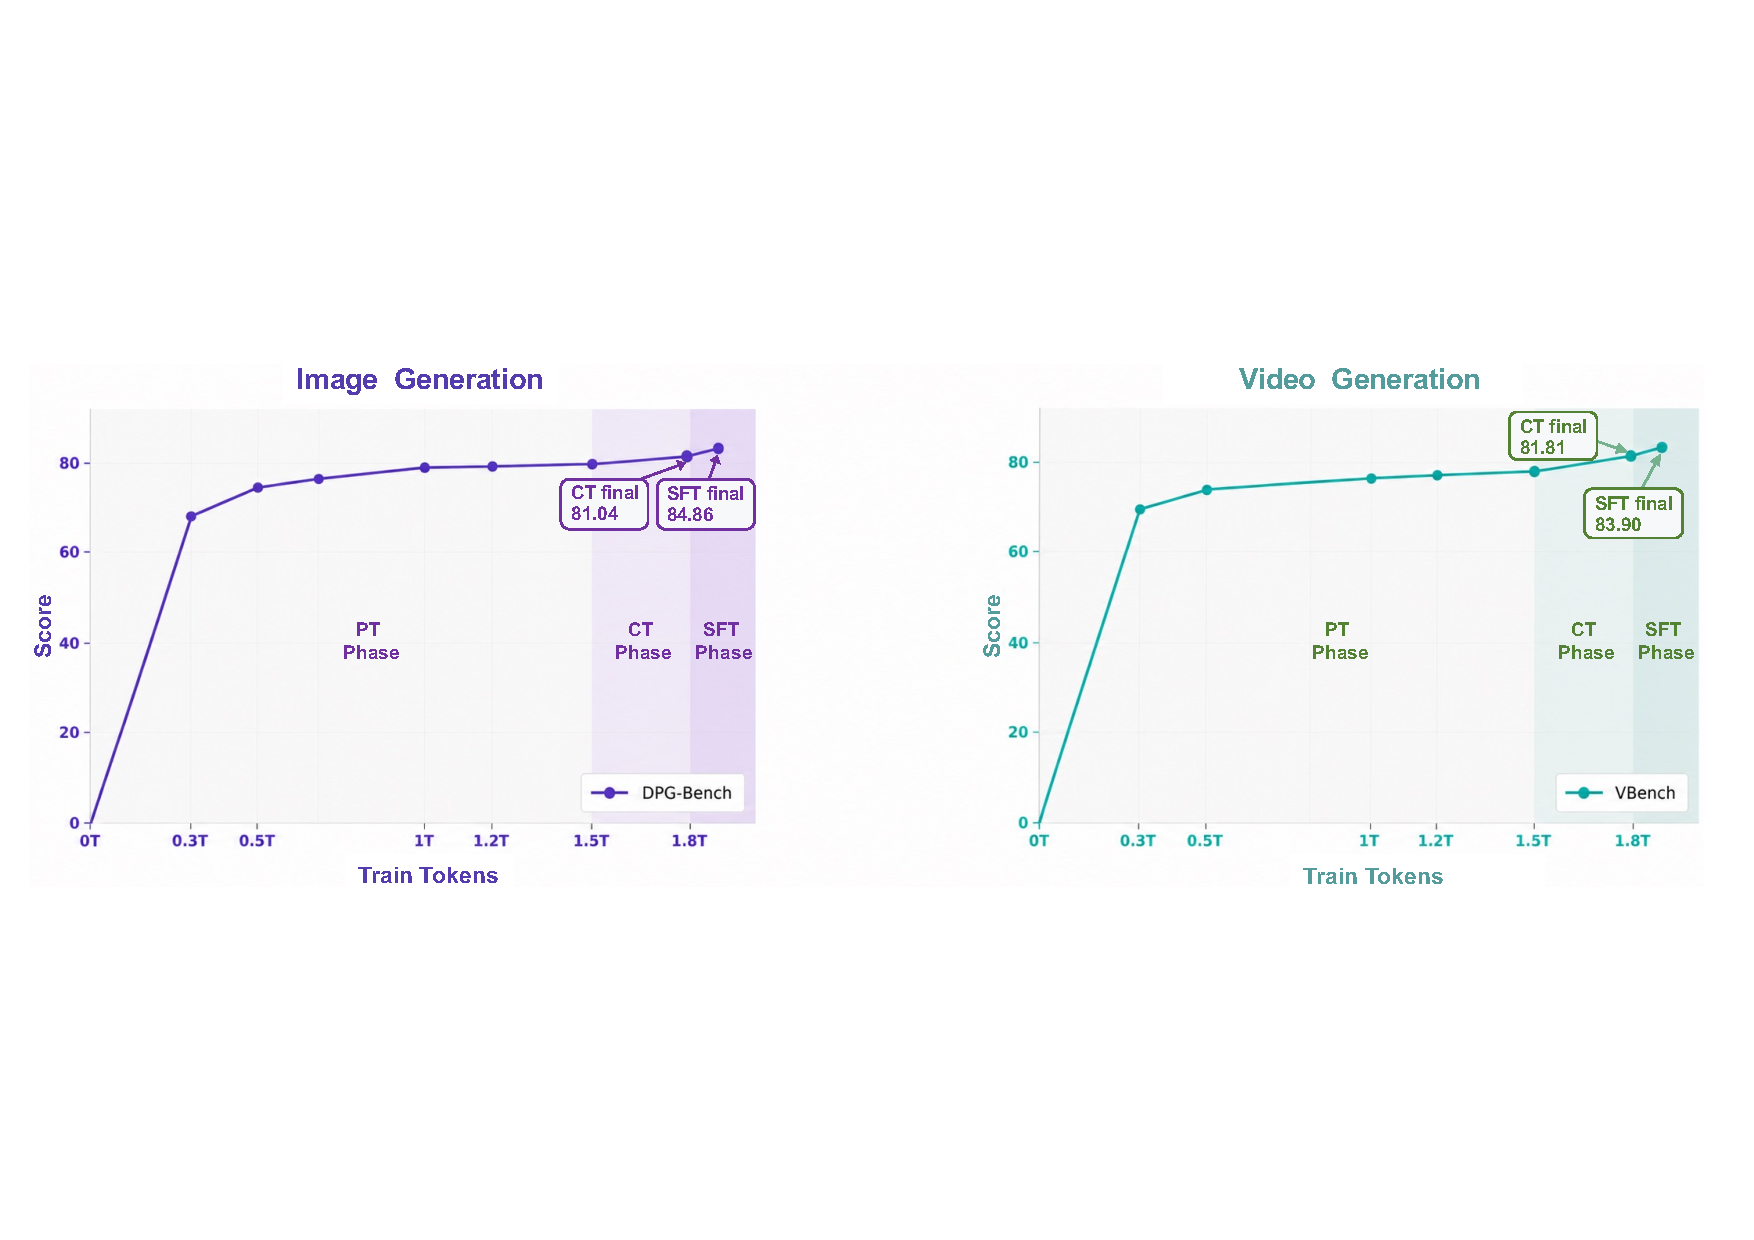
\includegraphics[width=1\textwidth]{figs/token-line.pdf}
    \caption{
    \textbf{Scaling behavior of image and video generation performance with increasing training tokens.}
    We report DPG-Bench for image generation and VBench for video generation across different training token budgets. 
    %The curves show that both benchmarks improve steadily as the token budget increases, with the CT and SFT phases highlighted separately. 
    % The 90\% performance point is marked for each benchmark, and the CT/SFT checkpoints further indicate the performance gains obtained during later-stage training.
    }
    \label{fig:token_scaling_curve}
\end{figure*}



\begin{figure*}[!t]
    \centering
    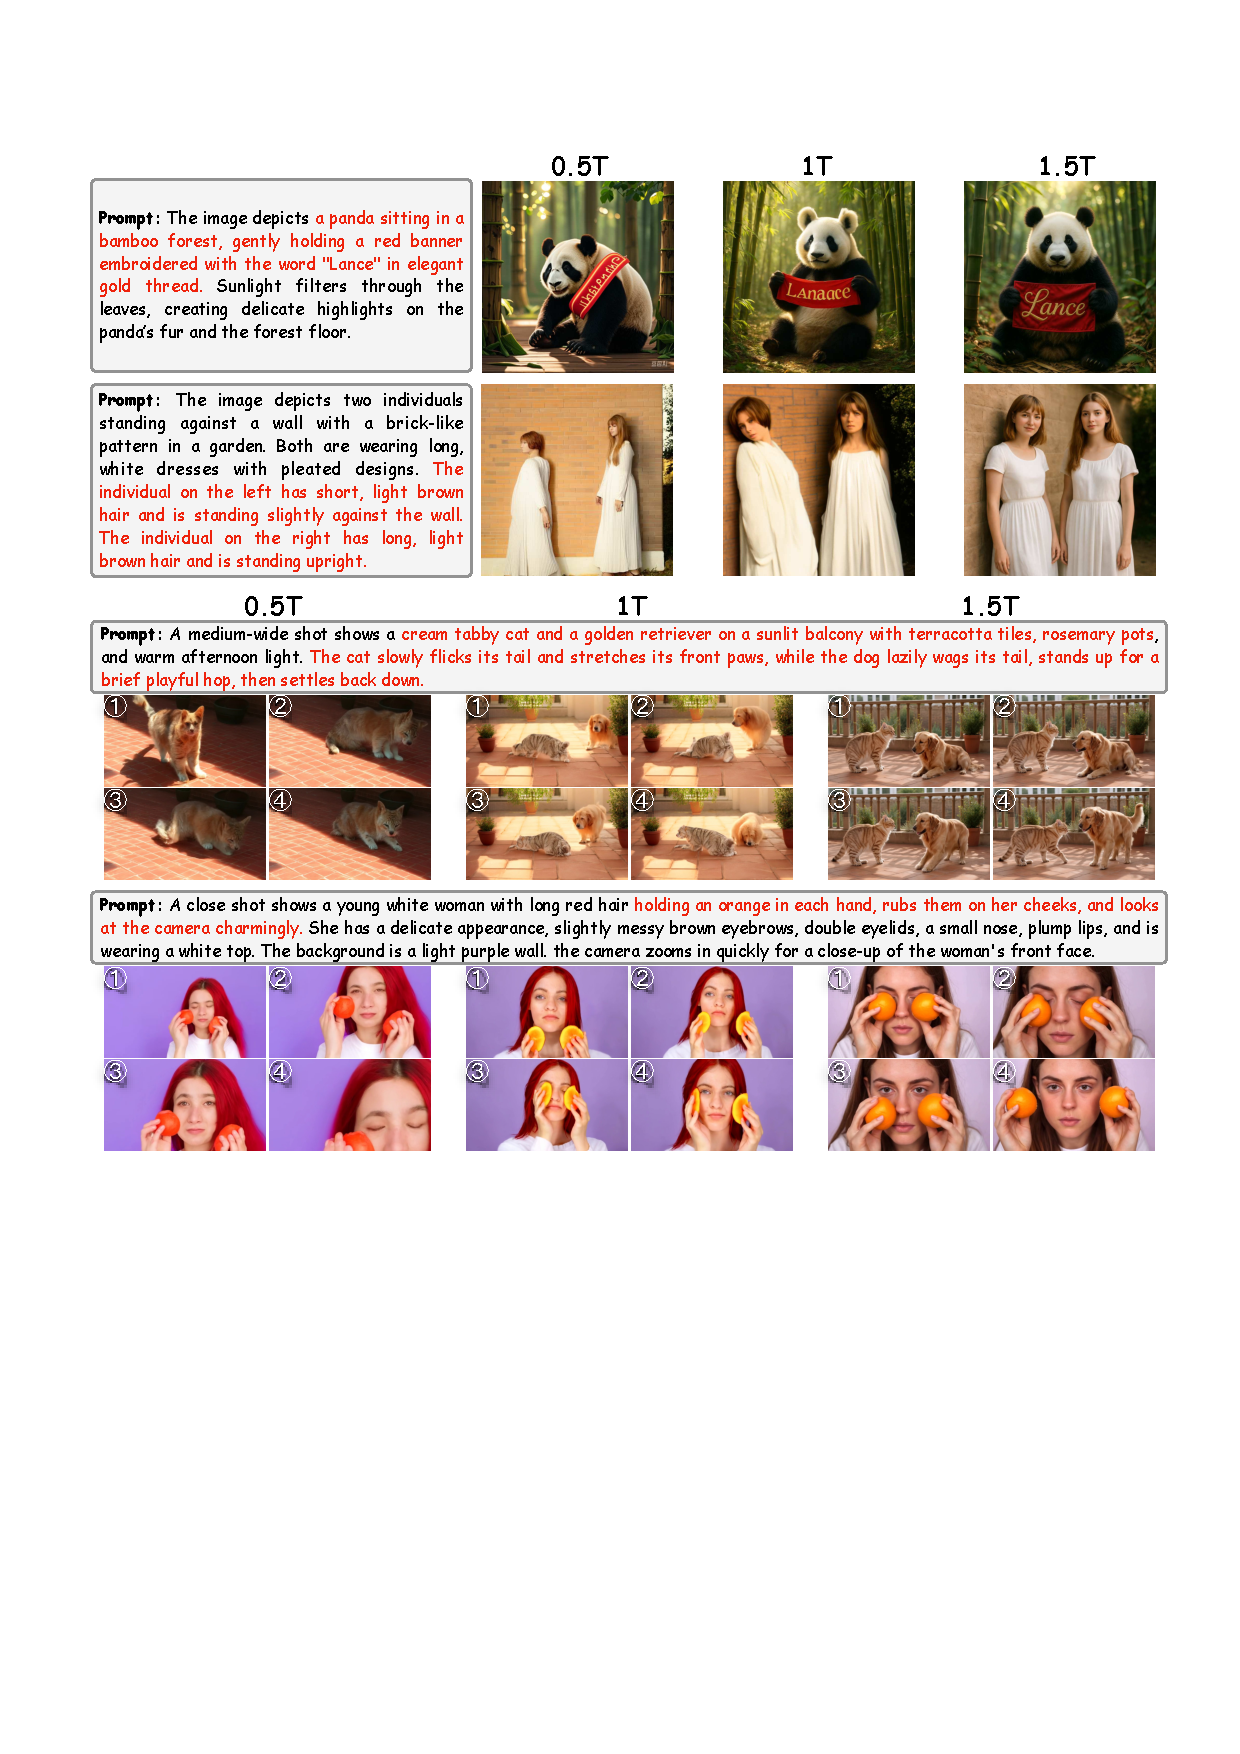
\includegraphics[width=1\textwidth]{figs/token-visual.pdf}
    \caption{
    \textbf{Comparison of model variants trained with different token budgets.}
    We present qualitative cases of text-to-image and video generation using model variants trained with $0.5$T, $1$T, and $1.5$T tokens. As the training budget increases, the model demonstrates improved prompt alignment, visual fidelity, and temporal consistency.
    }
    \label{fig:token_ablation}
\end{figure*}

\begin{table}[t]
\centering
\caption{\textbf{Ablation on cross-task data.} 
Gen. denotes base generation data, Und. denotes understanding data, and MT-Gen. denotes multi-task generation data, including editing, subject-driven generation, etc.
}
\label{tab:ablation_auxiliary_data_generation}
\setlength{\tabcolsep}{8pt}
\renewcommand{\arraystretch}{1.15}
\resizebox{1\linewidth}{!}{
\begin{tabular}{llccc}
\toprule
\multirow{2}{*}{\textbf{Ablation Type}} 
& \multirow{2}{*}{\textbf{Setting}}
& \multicolumn{1}{c}{\textbf{Image Generation}}
& \multicolumn{1}{c}{\textbf{Video Generation}}
& \multicolumn{1}{c}{\textbf{Video Understanding}} \\
\cmidrule(lr){3-3}
\cmidrule(lr){4-4}
\cmidrule(lr){5-5}
& 
& \textbf{GenEval $\uparrow$}
& \textbf{VBench $\uparrow$}
& \textbf{MVBench $\uparrow$} \\
\midrule

\rowcolor{rowblue}
\textbf{Base} 
& {Gen. only} 
& 80.88 
& 81.25 
& -- \\

\midrule

\multirow{2}{*}{\textbf{+ Understanding data}} 
& Gen.:Und. = 8:2 
& {81.65} 
& \underline{82.91} 
& 58.06 \\

& Gen.:Und. = 9:1 ({MT-Gen. Base})
& 80.93 
& 81.47 
& 57.99 \\

\midrule

\multirow{2}{*}{\textbf{+ Multi-task data}} 
& Gen.:Und. = 9:1, Gen.:MT-Gen. = 8:2  
& \underline{81.89} 
& 82.88 
& \textbf{59.18} \\

& Gen.:Und. = 9:1, Gen.:MT-Gen. = 6:4 
& \textbf{82.06} 
& \textbf{83.05} 
& \underline{58.95} \\

\bottomrule
\end{tabular}
}
\end{table}

\subsection{Training Dynamics Analysis}
To systematically analyze the evolution of model capabilities during training, we further conduct quantitative and qualitative evaluations of model variants under different training-token budgets.

\textbf{Quantitative Analysis.}
As shown in \Cref{fig:token_scaling_curve}, image and video generation exhibit broadly consistent scaling trends as training tokens increase, with rapid gains in the early PT stage followed by a slower-growth regime. This indicates that large-scale paired training first establishes core generation capability, while later tokens mainly refine prompt alignment, visual fidelity, and temporal consistency.
%: both improve rapidly at the early stage and then enter a slower-growth regime. Notably, image generation reaches the 90\% performance point earlier than video generation, requiring 0.67T tokens on DPG-Bench compared with 0.83T tokens on VBench, suggesting that video generation benefits from a longer training horizon due to its additional temporal modeling demands. 
Moreover, the CT stage further improves native generation capability, even though it mainly introduces multi-task data such as editing and instruction-following data rather than additional pure generation data (\Cref{tab:task_data_summary}). These results suggest that multi-task integration not only strengthens editing and instruction-following behaviors, but also brings positive transfer to visual generation, further validating the role of multi-task synergy in enhancing unified multimodal modeling.


\textbf{Qualitative Analysis.}
\Cref{fig:token_ablation} shows visual results consistent with the quantitative trends. As the training budget increases from $0.5$T to $1.5$T, Lance progressively improves prompt alignment, visual fidelity, text rendering, and temporal coherence. Early models capture coarse semantics but still suffer from distorted text, inaccurate attributes, and unstable motion, while the $1.5$T model produces more faithful compositions and more coherent multi-object dynamics. 




\subsection{Effect of Cross-Task Data Synergy}

We conduct ablation studies to further analyze how different task mixtures affect the generation and understanding ability of Lance, focusing on the effects of understanding data and multi-task generation data. 
%In particular, we focus on two questions: (1) whether incorporating understanding-oriented data benefits visual generation, and (2) whether incorporating multi-task generation learning improves base generation ability.
The results are summarized in \Cref{tab:ablation_auxiliary_data_generation}.


\textbf{Effect of Understanding Data.}
Introducing understanding-oriented data brings clear gains when used at an appropriate ratio. In particular, the Gen.:Und. = $8:2$ setting improves both image and video generation, suggesting that understanding data provides useful semantic grounding for visual synthesis. 

\textbf{Effect of Multi-task Data.}
Multi-task generation data enhances the base generation capability via joint training. Both mixture ratios outperform the generation-only baseline, with Gen.:MT-Gen. = $6:4$ achieving the best overall results. 
More unexpectedly, the benefits are not limited to generation: incorporating multi-task generation data also improves video understanding.
These results suggest that multi-task synergy is not merely a simple accumulation of capabilities, but may serve as an important mechanism for unlocking the further potential of unified models through mutual reinforcement across tasks.
% Overall, these results demonstrate that cross-task data can effectively strengthen generation. Understanding data mainly improves semantic grounding, while multi-task generation data further enhances visual synthesis through generation-oriented supervision.


%%%%%%%%%%%%%%%%%%

\subsection{Effect of Modality-Aware Rotary Positional Encoding}

We further ablate the proposed Modality-Aware Rotary Positional Encoding (MaPE) to verify its effectiveness in unified multimodal modeling. As shown in \Cref{tab:ablation_mape}, removing MaPE consistently degrades performance across generation, editing, and understanding. 
%These results demonstrate that explicitly separating heterogeneous visual token groups in the positional space is beneficial for unified multimodal modeling. 
The improvement is especially clear on image editing (from $6.30$ to $6.86$), where the model needs to jointly reason over visual conditions and generation targets. This suggests that MaPE reduces positional ambiguity among heterogeneous visual token groups, leading to better cross-task contextual alignment and more stable visual synthesis.


\begin{table}[t]
\centering
\caption{\textbf{Ablation on Modality-Aware Rotary Positional Encoding (MaPE).} We report GenEval for image generation, GEdit for image editing, VBench for video generation, and MVBench for video understanding.}
\label{tab:ablation_mape}
\setlength{\tabcolsep}{8pt}
\renewcommand{\arraystretch}{1.15}
\resizebox{0.8\linewidth}{!}{
\begin{tabular}{lcccc}
\toprule
\multirow{2}{*}{\textbf{Setting}} 
& \multicolumn{1}{c}{\textbf{Image Generation}} 
& \multicolumn{1}{c}{\textbf{Image Editing}} 
& \multicolumn{1}{c}{\textbf{Video Generation}} & \multicolumn{1}{c}{\textbf{Video Understanding}} \\
\cmidrule(lr){2-2} \cmidrule(lr){3-3} \cmidrule(lr){4-4} \cmidrule(lr){5-5}
& \textbf{GenEval $\uparrow$} & \textbf{GEdit $\uparrow$} & \textbf{VBench $\uparrow$} &\textbf{MVBench $\uparrow$} \\
\midrule
\rowcolor{rowblue}
\textbf{w/ MaPE} & \textbf{80.94} & \textbf{6.86} & \textbf{81.81} &\textbf{59.16} \\
\textbf{w/o MaPE} & 80.56 & 6.30 & 80.95 & 59.02 \\
\bottomrule
\end{tabular}
}
\end{table}